\chapter{The LHC and ATLAS experiments} \label{chap:LHCAtlas}

\section{The LHC} \label{sec:LHC}
The Large Hadron Collider (LHC), with its 27 kilometres ring \cite{LHCguide}, is the world largest particle accelerator. It is part of the CERN’s accelerator complex and it is situated around 100 metres underground to shield from radiation and for both economic\footnotemark and geological reasons. With its first run on 10 September 2008, it currently accelerates hadrons, in particular protons or lead nuclei. The LHC is composed by two circular beam pipes where two particle beams travel separately in opposite direction, close to the speed of light. Due to the very high speed, when the two beams collide, the energy of the center of mass, known as $\sqrt{s}$, is twice the energy of each beam (which is the same). In fact, knowing that $E^2=m^2c^4+p^2c^2$ and using the natural unit system ([m]=eV/$c^2$, [p]=eV/c), we get: $E^2=m^2+p^2\simeq p^2$, where at the end an ultra-relativistic particle (p>>m) was assumed. This information is used in the norm of the four-momentum of two colliding particles \cite{Bini}:
\begin{equation}\label{eq:centerofmasseq}
    \sqrt{s}=\sqrt{P_{\mu}P^{\mu}}=\sqrt{E_{tot}^2-|\Vec{p_{tot}}|^2}=\sqrt{(E_1+E_2)^2-|\Vec{p_1}-\Vec{p_2}|^2}\simeq 2 E
\end{equation}


\noindent where we assumed $E_1$ = $E_2$. At the LHC protons are accelerated with an energy of 6.8 TeV ($10^{12}$ eV), which confirms the assumption p>>m and it leads to $\sqrt{s}=13.6$ TeV \cite{LHCreport}. Such high energies are reached through a series of increasing accelerators, shown in figure \ref{fig:LHCaccelerators}, where Radio-frequency cavities accelerate particles, through an oscillating electric field.\\
Accelerated beams are directed and curved by superconducting electromagnets with a magnetic field of up to 8.3 T \cite{PhDFrattari}: 1232 dipole magnets and 392 quadrupole magnets are used. Although its huge contribution, magnetic field also represents one of the main limitations of this apparatus. In fact from the Lorentz force $\Vec{F}=q(\Vec{E}+\Vec{v}\times \Vec{B})$, it is possible to get a connection between external magnetic field $\Vec{B}$, particle momentum and its radius of curvature, which is \cite{Bini}:
\begin{equation}\label{eq:pqBR}
    p = qBR
\end{equation}

\noindent where q is the charge of the particle and R the radius of curvature. It is evident that, working with high energy particles, to reduce R we need to generate a bigger magnetic field, but current technologies set a limit to this value.
\footnotetext{Building LHC on the surface would have required the purchase of properties to do so and an under the open sky structure with a 27 km circumference would have been more expensive than agreeing with landowner and excavate a tunnel underground.}

\noindent Performance of the LHC are evaluated based on an essential parameter: the instantaneous luminosity $\mathcal{L}$, measured in $cm^{-2}s^{-1}$ and computed as follows \cite{LHCreport}.
\begin{equation}\label{eq:Luminosity}
    \mathcal{L}=\frac{N_b^2n_bf_{rev}\gamma_r}{4 \pi \epsilon_n \beta^*}F
\end{equation}

\noindent where: $N_b$ is the number of particles in a bunch, $n_b$ is the number of bunches in a beam, $\epsilon_n$ is the normalized transverse beam emittance, $\beta^*$ is the beta function at the collision point, $\gamma_r$ is the relativistic factor, $f_{rev}$ is the revolution frequency. F represents the geometric luminosity reduction factor:
\begin{equation}
    F=\frac{1}{\sqrt{1+\Big(\frac{\theta_c\sigma_z}{2\sigma^*}\Big)^2}}
\end{equation}
\noindent where $\theta_c$ is the full crossing angle at the interaction point, $\sigma_z$ is the RMS bunch length and $\sigma^*$ is the transverse RMS beam size at the interaction point. Luminosity is linked with the number of collisions per second \cite{Bini}:
\begin{equation}\label{eq:dNdt}
    \frac{dN}{dt}=\mathcal{L}\sigma_{tot}
\end{equation}
\noindent where $\sigma_{tot}$ is the total cross section. If the
instantaneous luminosity goes below a fixed threshold, beams are dumped.


\begin{figure}
    \centering
    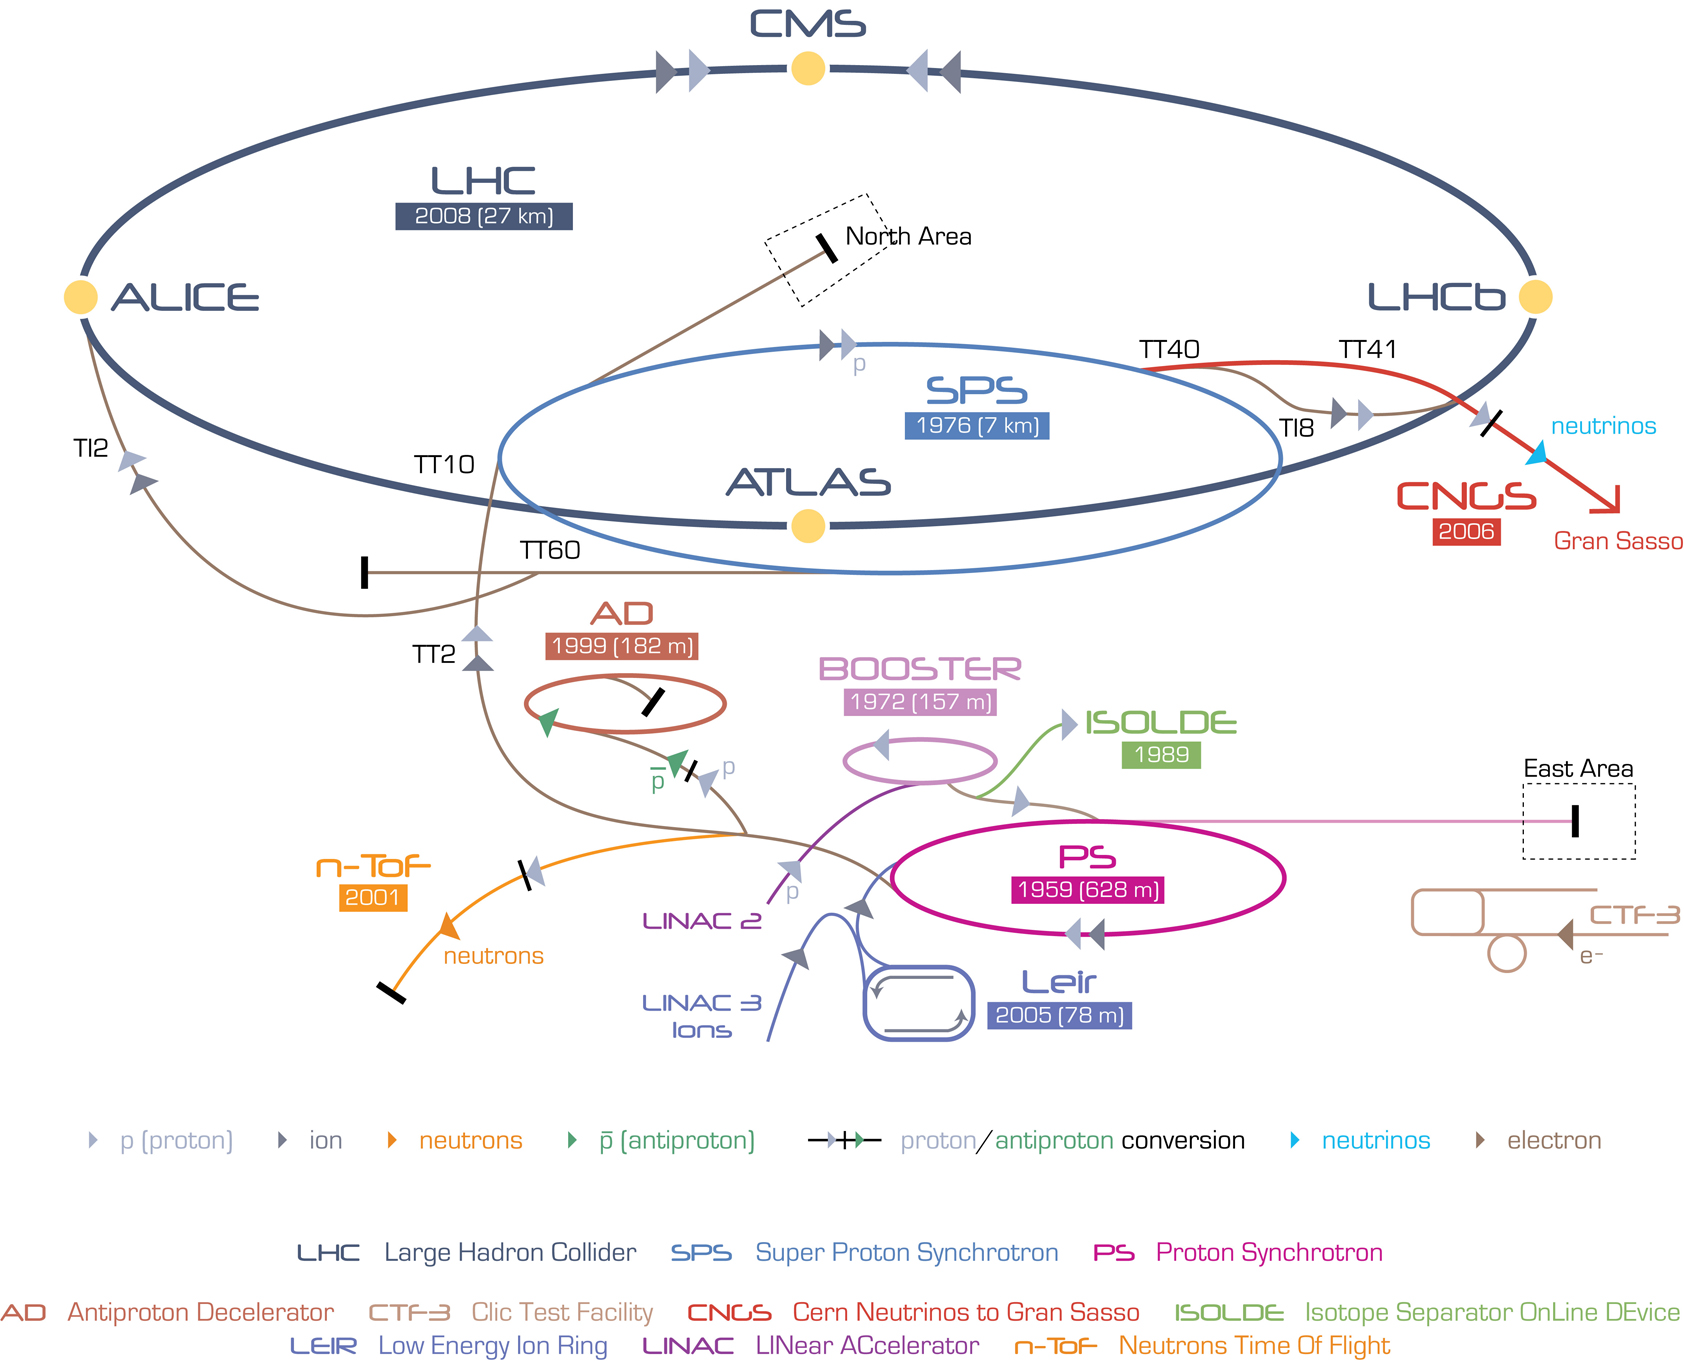
\includegraphics[width=3 in]{OLD/Images/Cap2/LHCaccelerators.png}
    \caption{CERN accelerating system. Figure from Ref. \cite{PhDFrattari}}
    \label{fig:LHCaccelerators}
\end{figure}


%%%%%%%%%%%%%%%%%%%%%%%%%%%%%%%%%%
\section{ATLAS}\label{sec:ATLAS}
A Toroidal LHC ApparatuS (ATLAS) \cite{ATLASwebsite} is the world largest particle detector, situated at interaction point 1 at CERN. It has many layers in a cylindrical symmetry around the beam pipe. 44m in length and 25m in height are required to investigate collisions between particles accelerated by LHC, to study phenomena such dark matter, the Higgs boson and top quark. The main components of the detector are: an inner detector, an electromagnetic and a hadronic calorimeter, and the muon spectrometer, as shown in Figure \ref{fig:ATLASdetector}.\\
The inner detector relies on a 2 T solenoidal magnetic field, parallel to the beam axis, to 
reconstruct the tracks of charged particles. This information is used to measure the momentum of them using the sagitta method and the relation between momentum and radius of curvature, presented in (\ref{eq:pqBR}).\\
The electromagnetic calorimeter \cite{ATLASexp} measures the energy of electrons, photons and hadrons. Once a particle among them hits the detector, an electromagnetic shower is generated and the energy of the particle is transferred to the material through radiation, as shown in figure \ref{fig:EMShower}. Passive components of the calorimeter such as lead induce the loss of energy and the active ones, made by Liquid Argon (LAr) kept at a temperature of -184 °C, measure it. The shower is fully contained in this part of the detector, which is longer then 20 radiation lengths. For this reason this technique to measure energy is defined \textit{destructive}.\\

\begin{figure}[h!]
    \centering
    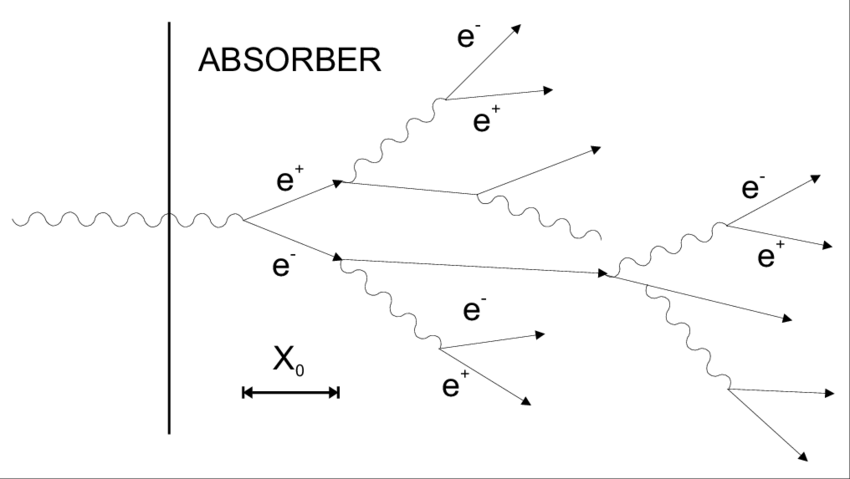
\includegraphics[width=3 in]{OLD/Images/Cap2/EMShower.png}
    \caption{Schematic of an electromagnetic shower starting from a photon}
    \label{fig:EMShower}
\end{figure}

\noindent The hadronic calorimeter has been placed to measure the energy of hadrons that survive to the electromagnetic calorimeter. It relies on the principle of particle shower, which is converted into an electric current and measured.\\
The muon spectrometer is the last component of the ATLAS experiment and measures the momenta of muons. In fact, they are similar to electrons, but with a greater mass, which leads only to weak interactions and more depth of penetration. This is why they are not revealed by inner systems.\\
The coordinate system adopted at ATLAS to describe events is discussed in detail in section \ref{sec:CoordinateSystem}.

\begin{figure}
    \centering
    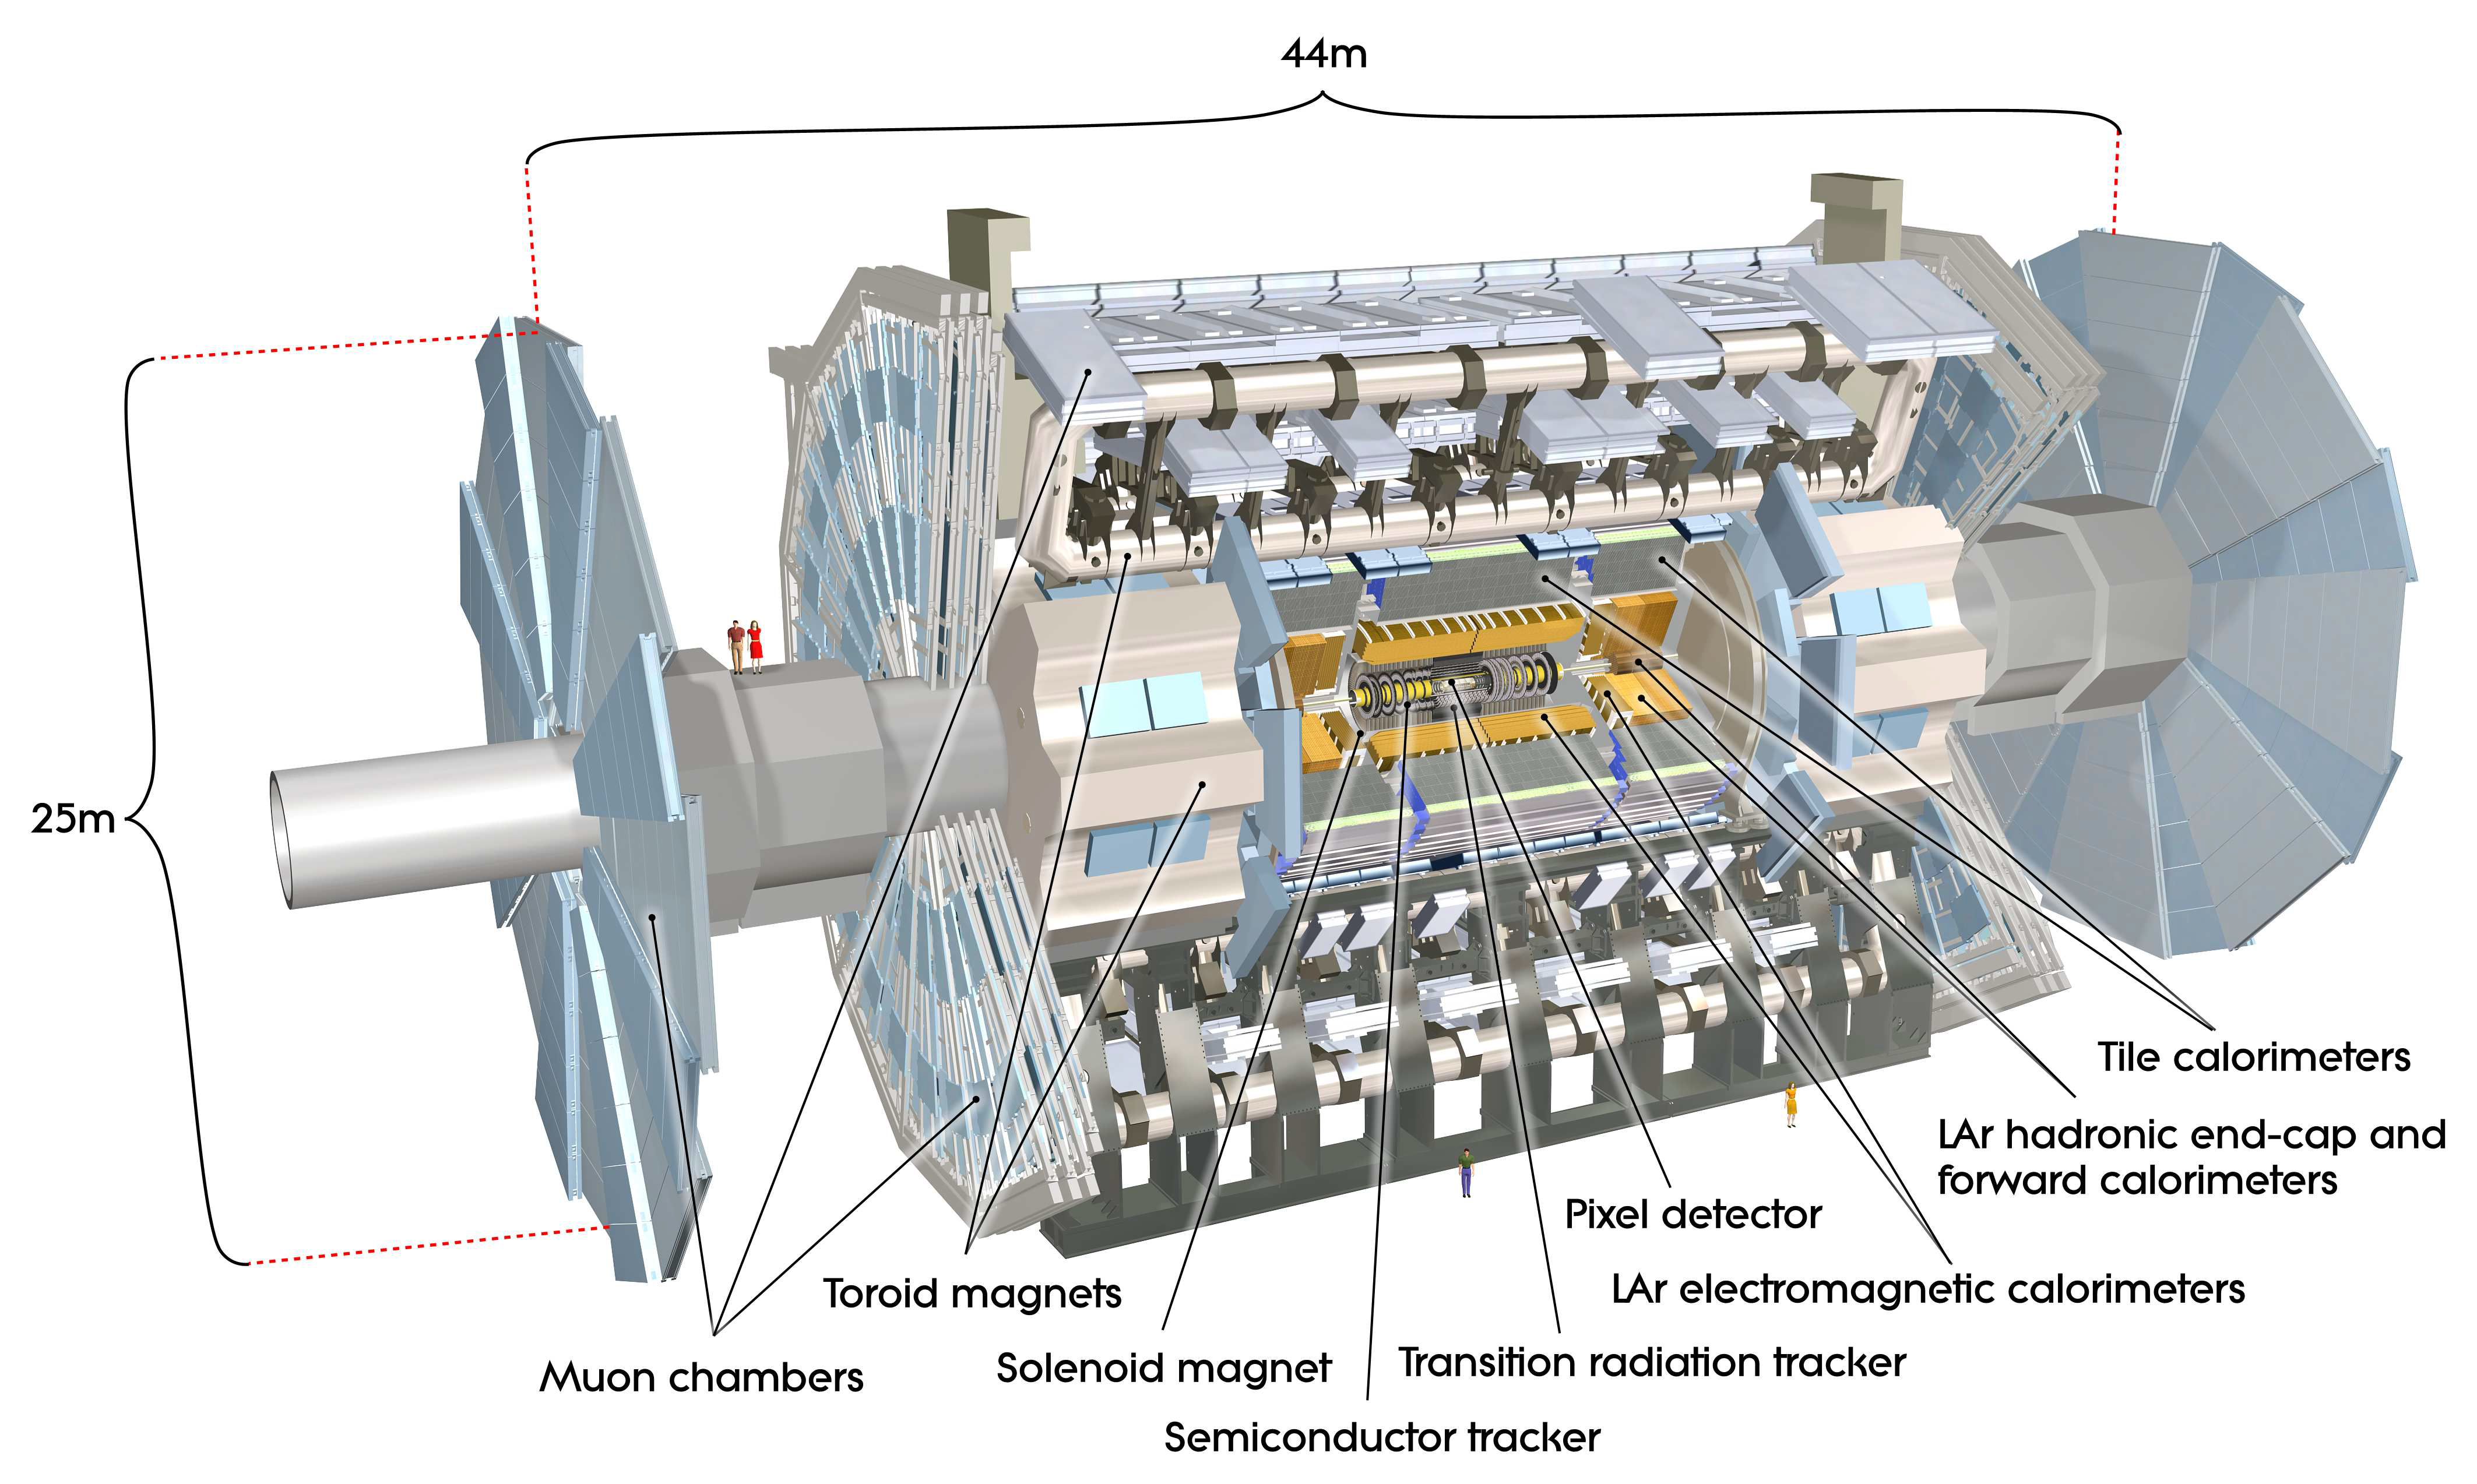
\includegraphics[width=3.5 in]{OLD/Images/Cap2/ATLASdetector.png}
    \caption{ATLAS schematic. Figure form Ref. \cite{ATLASexp}}
    \label{fig:ATLASdetector}
\end{figure}


%%%%%%%%%%%%%%%%%%%%%%%%%%%%%%%%%%
\section{Problems in Particle Physics}\label{sec:problemsHEP}
The 20th century was a golden era in Particle Physics, due to the high number of discoveries happening during it. Thanks to them we now have a complete overview of how the subatomic world works. The overview was completed in 2012 with the first observation of the Higgs boson. Everything we know is contained in the Standard Model of particle physics\cite{SMCern}: 6 quarks (up, down, charm, strange, top, bottom), 6 leptons (electron, muon, tau and corresponding neutrinos), 4 bosons that mediate the 4 fundamental forces (strong, weak, electromagnetic, gravitational) and the Higgs boson giving them a mass by the homonymous mechanism. The SM describes very well these phenomena but there are still many problems that need to be solved.\\
\begin{figure}[h!]
    \centering
    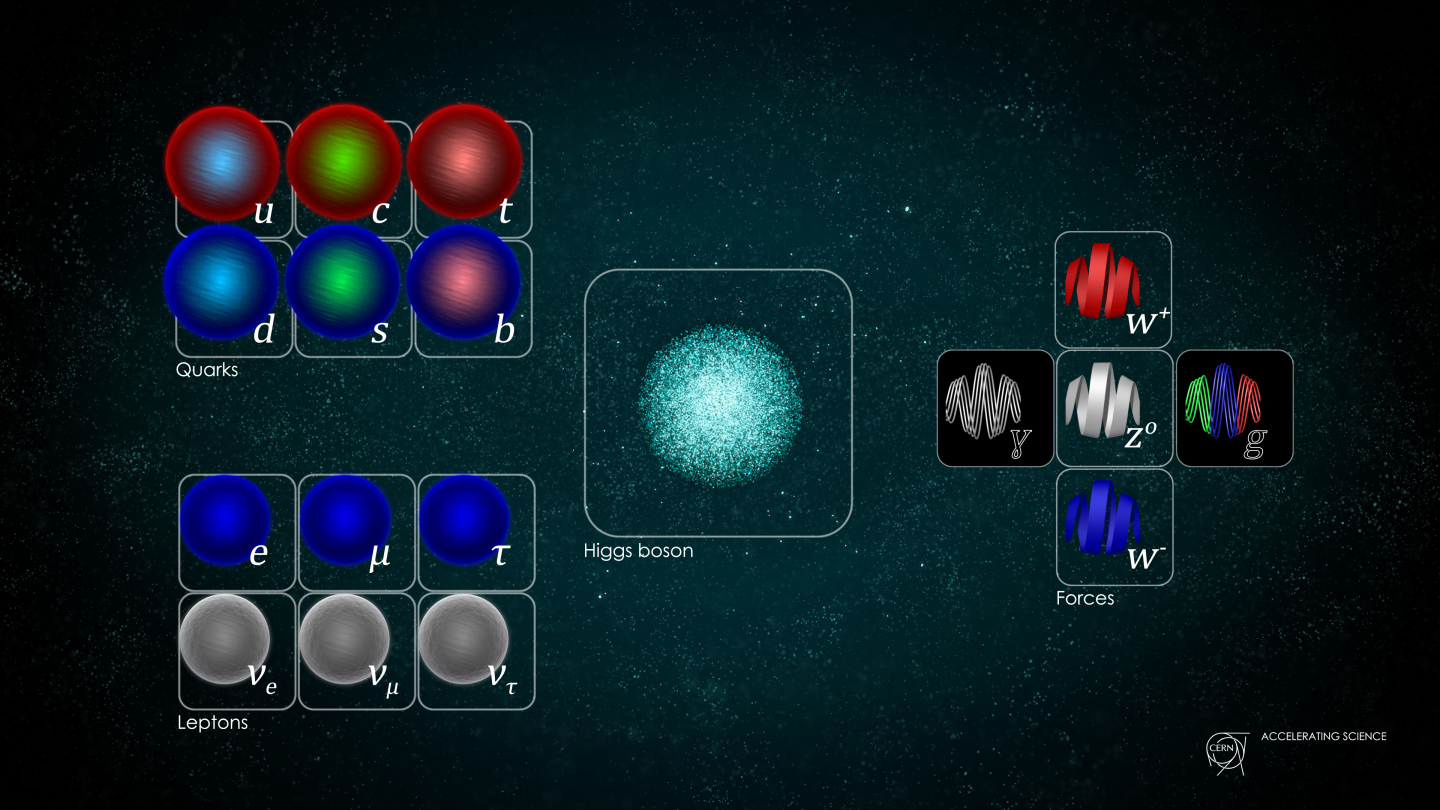
\includegraphics[width=3 in]{OLD/Images/Cap2/SMpicture.png}
    \caption{Particles of the Standard Model. Figure from Ref. \cite{SMCern}}
    \label{fig:SMpicture}
\end{figure}

\noindent Among all unsolved mysteries, we can find: unification of gravitational interaction and other interactions, the mass of neutrinos, the baryon - anti-baryon asymmetry in the Universe and Dark Matter. In particular the last is giving physicists a hard time. From cosmological observation it is known that ordinary matter constitutes only 5\% of the mass of the Universe, 27\% is Dark Matter and 68\% is Dark Energy. If we investigate the last two using particle accelerators, we expect them to leave the experiment undetected due to their low ratio of interactions and then from missing energy we can observe their presence. Anyway, using traditional data analysis techniques, they have not been observed yet on the Earth. One possible explanation for this "failure" could be the limits of model depending theoretical model used. In this situation a model agnostic approach such as Anomaly Detection comes to help.





